% Capítulo 11: lista encadeada e a remoção do nó 30 religando os ponteiros.
\documentclass[border=4pt]{standalone}
\usepackage[utf8]{inputenc}
\usepackage[T1]{fontenc}
% Estilo comum das figuras de vetores (capítulo 8).
\usepackage{tikz}
\usetikzlibrary{arrows.meta, positioning, calc, decorations.pathreplacing}
\definecolor{navy}{RGB}{23,45,80}
\definecolor{laranja}{RGB}{250,110,29}
\definecolor{cinzalogo}{RGB}{107,114,126}
\definecolor{azul}{RGB}{205,222,247}
\tikzset{
  casa/.style={draw=navy, line width=0.9pt, minimum width=8mm, minimum height=7mm,
               inner sep=0pt, font=\sffamily\small},
  pronta/.style={casa, fill=azul},
  parte/.style={casa, fill=laranja!12},
  marcada/.style={casa, fill=laranja!45, draw=laranja},
  fora/.style={casa, draw=cinzalogo!60, dashed, fill=white, text=cinzalogo!60},
  indice/.style={font=\sffamily\scriptsize, text=cinzalogo},
  explica/.style={font=\sffamily\small, text=navy, anchor=east},
  legenda/.style={font=\sffamily\scriptsize, text=cinzalogo},
  rotulo/.style={font=\sffamily\small\bfseries, text=navy},
  seta/.style={-{Stealth[length=2.2mm]}, navy, line width=0.9pt},
  chave/.style={decorate, decoration={brace, amplitude=4pt, mirror}, navy, line width=0.8pt},
}
% \vetor{nome}{x}{y}{valor/estilo, valor/estilo, ...}: casas lado a lado, chamadas nome0, nome1...
\newcommand{\vetor}[4]{%
  \foreach \valor/\estilo [count=\i from 0] in {#4} {
    \node[\estilo] (#1\i) at ($(#2, #3) + (\i*0.8, 0)$) {\valor};
  }
}

\usetikzlibrary{shapes.multipart}
\tikzset{
  no/.style={rectangle split, rectangle split horizontal, rectangle split parts=2, draw=navy, line width=0.9pt,
             fill=azul, font=\sffamily\small, minimum height=7mm, inner sep=3pt,
             rectangle split part fill={azul, white}},
  noremovido/.style={no, draw=cinzalogo!70, dashed, rectangle split part fill={white, white}, text=cinzalogo},
  liga/.style={-{Stealth[length=2.2mm]}, navy, line width=0.9pt},
  nulo/.style={font=\ttfamily\scriptsize, text=cinzalogo},
}
\begin{document}
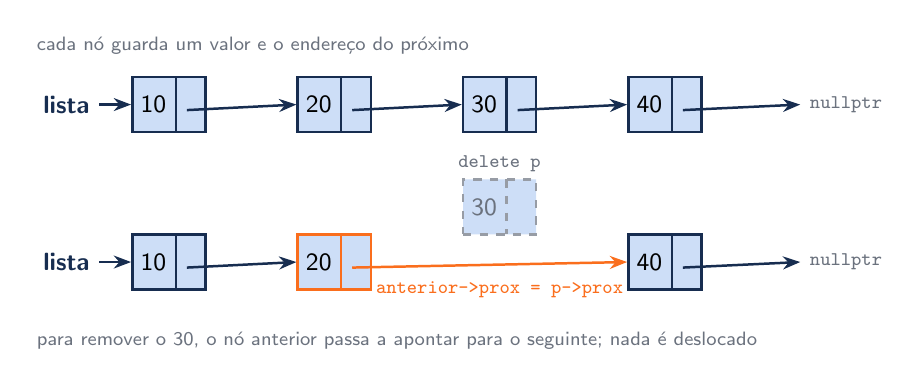
\begin{tikzpicture}
  % lista original
  \node[rotulo] (L1) at (-1.3, 0) {lista};
  \foreach \v [count=\i from 0] in {10, 20, 30, 40} {
    \node[no] (a\i) at (\i*2.1, 0) {\v \nodepart{two} \phantom{x}};
  }
  \node[nulo] (n1) at (8.6, 0) {nullptr};
  \draw[liga] (L1) -- (a0.west);
  \foreach \i/\j in {0/1, 1/2, 2/3} {
    \draw[liga] ($(a\i.two)+(0.02, 0)$) -- (a\j.west);
  }
  \draw[liga] ($(a3.two)+(0.02, 0)$) -- (n1.west);
  \node[legenda, anchor=west] at (-1.8, 0.75) {cada nó guarda um valor e o endereço do próximo};

  % depois de remover o 30
  \node[rotulo] (L2) at (-1.3, -2.0) {lista};
  \node[no] (b0) at (0, -2.0) {10 \nodepart{two} \phantom{x}};
  \node[no, draw=laranja] (b1) at (2.1, -2.0) {20 \nodepart{two} \phantom{x}};
  \node[noremovido] (b2) at (4.2, -1.3) {30 \nodepart{two} \phantom{x}};
  \node[no] (b3) at (6.3, -2.0) {40 \nodepart{two} \phantom{x}};
  \node[nulo] (n2) at (8.6, -2.0) {nullptr};
  \draw[liga] (L2) -- (b0.west);
  \draw[liga] ($(b0.two)+(0.02, 0)$) -- (b1.west);
  \draw[liga, laranja] ($(b1.two)+(0.02, 0)$) -- (b3.west);
  \draw[liga] ($(b3.two)+(0.02, 0)$) -- (n2.west);
  \node[legenda, text=laranja] at (4.2, -2.35) {\texttt{anterior->prox = p->prox}};
  \node[legenda] at (4.2, -0.75) {\texttt{delete p}};
  \node[legenda, anchor=west] at (-1.8, -3.0) {para remover o 30, o nó anterior passa a apontar para o seguinte; nada é deslocado};
\end{tikzpicture}
\end{document}
